\documentclass[conference]{IEEEtran}
\IEEEoverridecommandlockouts
% The preceding line is only needed to identify funding in the first footnote. If that is unneeded, please comment it out.
\usepackage{cite}
\usepackage{amsmath,amssymb,amsfonts}
\usepackage{algorithmic}
\usepackage{graphicx}
\usepackage{textcomp}
\usepackage{xcolor}
\def\BibTeX{{\rm B\kern-.05em{\sc i\kern-.025em b}\kern-.08em
    T\kern-.1667em\lower.7ex\hbox{E}\kern-.125emX}}
\begin{document}
\begin{titlepage}

\title{Sharing and Binding for General Circuits\\}

\author{\IEEEauthorblockN{Benedikt Lipinski}
\IEEEauthorblockA{\textit{Interaktionstechnik und Design} \\
\textit{Hochschule Hamm Lippstadt}\\
Lippstadt, Germany \\
benedikt.lipinski@stud.hshl.de}
}
\maketitle
\begin{abstract}

\end{abstract}
\end{titlepage}


\newpage
\section{Introduction}
Durch das menschliche Verlangen, Problemstellungen zugunsten schwindender Komplexität und erhöhten Komforts zu automatisieren und zu brechen, wurden genau diese Anforderungen auf diejenigen elektrischer Schaltungen umgelegt. 
\subsection{Problemstellung}
Nicht erst durch moderne Entwicklungen wie digitale Vernetzung mit dem Internet der Dinge  oder das autonome Fahren wird die Betrachtung zeitlicher und finanzieller Aspekte für die Entwicklung multidimensionaler Systeme notwendig. Allerdings lassen genau diese Entwicklungen die Komplexität sprunghaft ansteigen.

\subsection{Logische Bausteine}
Realisierbar werden elektrische Verschaltungen in der Digitaltechnik erst durch den Einsatz sogenannter Logikbausteine, die miteinander kombiniert ein vorher genau bestimmtes Verhalten der geplanten Schaltung verursachen.
Hierbei übernehmen verschiedene Bausteine verschiedene Aufgaben, die mal weniger und mal mehr komplizierte Operationen beinhalten. 
\subsubsection{AND-Gatter}
Eine der Grundoperationen, die in fast jeder Schaltung zu finden ist, ist die AND-Operation, zu deutsch die UND-Operation. Hierbei wird der Eingang erst auf logisch 1 geschaltet, wenn alle Eingänge dies ebenfalls sind.\\
\begin{tabular}[h]{ccc}
x&y&Out\\
0&0&0\\
0&1&0\\
1&0&0\\
1&1&1\\
\end{tabular}
\subsubsection{OR-Gatter}
Das Ergebnis des OR-Gatters ist in dem Fall wahr, wenn einer seiner Eingänge wahr ist.\\
\begin{tabular}[h]{ccc}
x&y&Out\\
0&0&0\\
0&1&1\\
1&0&1\\
1&1&1\\
\end{tabular}
\\Simple Schaltungen lassen sich durch das gezielte Aneinanderreihen von AND- und OR-Gattern gut realisieren, sollte aber 
\subsubsection{Multiplexer}
Multiplexer werden genutzt, wenn eine parallele Verarbeitung aus unterschiedlichsten Gründen nicht möglich ist. Das kann zum einen eine nicht ausreichende Verfügbarkeit an Kanälen sein, aber auch die bewusste Entscheidung, weniger Kanäle aus Kostengründen zu benutzen, sein. Dieser Schritt kann gewählt werden, wenn Verläufe zwar parallel laufen, aber nur exklusiv ausgeführt werden. Das bedeutet, dass nach einer elementaren Entscheidung nur einer der beiden Stränge ausgeführt werden kann. Beeindruckend allerdings ist, dass Multiplexer trotz ihrer fortgeschrittenen Eigenschaften gegenüber der Grundbausteine doch recht simpel aus genau diesem erzeugt werden können. So ergibt sich für einen einfachen Multiplexer das Schaltbild aus zwei AND-Gattern, einem NOT-Gatter und einem OR- Gatter. .....
\subsubsection{FPGA}
Der Einsatz von diesen Grundelementen ist für das Erreichen des Ziels völlig hinreichend, doch benötigen sie eine sehr hohe Fläche, auf der sie verbaut werden müssen. Ein zu erreichendes Ziel ist, die Fläche auf der die Schaltung realisiert werden muss, zu verringern. Dies ist durch die Verwendung von Halbleitern und die Entwicklung von integrierten Schaltkreisen auch erfolgreich gelungen, allerdings besitzen diese sogenannten ICs den Nachteil, dass ihre Schaltung- wie die einer Realisierung mit Bausteinen- auch fest gebunden ist. Ein Nachteil, den FPGA (Field Programmable Gate ARRAY) Bauteile nicht besitzen, ihr Vorteil ist die Zusammensetzung aus zusammengeschalteten Baugruppen aus Logikbausteinen, FlipFlops und deren Verbindung mit Multiplexern. In FPGAs kann das Verhalten der Eingänge zu den Ausgängen über{\color{red}...... }"programmiert" werden.
\subsection{Strategien zur Architektur-Optimierung}
Mit steigender Komplexität der Verschaltungen steigt zwingend auch die Anzahl der  zu nutzenden Bauteile. Zudem steigt auch die Verwendung performaterer Bausteine stetig, um die Abarbeitung bezüglich Leistung und aller zeitlichen Deadlines einhalten zu können. Nachteilig ist vor dem Hintergrund ebenfalls, dass Bausteine mit einer höheren Leistung oftmals auch einen erhöhten Platzbedarf einfordern\cite[S.327]{2}.\\
Ziel ist es, Strategien umzusetzen, die die Chipfläche verringern, ohne dabei die Leistungsfähigkeit der Schaltung zu beeinflussen. Leider ist dieses Problem nicht mit der Einhaltung beider Anforderungen zu vereinbaren, wodurch zum Beispiel die Verminderung der Kosten durch Senkung der Chip-Anzahl und Fläche immer auch zum Nachteil der Performance agiert. Der Zusammenhang zwischen Fläche und der erzeugten Leistungsverminderung ergibt sich aus der Fläche $a$ in der Einheit Gatteräquivalent $(Gate Equivalent GE)$, das die Größe des simpelsten Gatters widerspiegelt\cite[S.326]{2} und der Performance, die den Kehrwert der Ausführungszeit $T_{ges}$ widerspiegelt $\frac{1}{T_{ges}}$, die sich wieder aus der Taktzeit $T_c$ multipliziert mit der Latenz $\lambda$ zusammensetzt
\cite[S.325-326]{2}.\\
 Eine mögliche Realisierung der Schaltung mit einer bestimmten Performance bei einer bestimmten Fläche lässt sich als Punkt in einem Diagramm darstellen, dessen Achsen sowohl die Chipfläche, die Latenz und den Takt abbilden\cite[S.326]{2}.
 Dieses Vorgehen\cite{?} ist in diesem Fall notwendig, da mehr als eine Variable optimiert werden muss, und es dementsprechend mehr als eine gültige Lösung dieses Problems gibt. Als mögliches Hilfsmittel kann hier die Pareto-Optimierung verwendet werden. Die Pareto-Optimierung erzeugt eine Kompromisslösung durch die Gewichtung jeder Einzelfunktion. Die Idee dahinter ist, dass die Gewichtung die Wichtigkeit der Einzelfunktion repräsentiert und ihr bei steigendem Gewicht mehr Aufmerksamkeit verleiht\cite[S.45]{4}. Als ergebnis erhalten wir sogenannte Pareto punkte, diese punkte in unserem entwurfsraum stellen verschiedenste verhältnisse unserer optimierungs variablen dar. Eine Pareto optimale lösung, ist die lösung, die gülltig gegenüber aller gestellten anforderungen ist und die das best mögliche ergebnis aller variablen liefert, ohne das sich eine verschlechtert nur um eine andere weiter zu optimieren.

\subsection{Allocation}

%...ist eigl. Binding wird aber auch mit der betrachtung der zur verfügung stehenden Resourcen in verbinduggebracht 

%MEnge der zur Verfügung stehenden recourcen 
%Die Allokation ist eine Funktion, die angibt zu welchem Ressourcen typ Wiviele REssourcen zu r verfügung stehen 




Nicht nur, aber vor allem aus Kosten und Platzgründen stehen der Entwicklung selten unbegrenzte resourcen zur verfügung. Aus diesem Grund kann die Betrachtung der zur verfügung stehenden resourcen zwingend notwendig werden. Somit ist das ergebnis der allokierung nach Teich \cite{1}    
, eine funktion $ \alpha(r_k)$ die angibt wie viele verfügbare Bauteile es zu einer Jeweiligen Resourcentyp gibt.\\
Damit würde, wenn vom Resourcentyp Mulitplizier: $r_1$,Beispielweise 1 Einheiten zur verfügung stehen die Allokierungsfunkion $\alpha(r_1) = 2$ lauten. Die Funktion der Allokation zeigt deshalb ziemlich genau welche probleme beziehungsweise zeitliche veränderungen entstehen durch die grenzen, die durch die begrenzte verfügbarkeit an Resourcen gegeben werden. Dies kann ein nützlicher zwischenschritt sein um den überblick zu behalten,den Teich mittels eines Ressourcen graphen anschaulich darstellt.In vielen Literaturen allerdings wird dieser schritt auch in die Bindung integriert und nicht extra behaldelt.
\subsection{Binding}
Im unterschied zur Allokierung wird in der Bindung schließlich festgelegt welche Resource welche operation zugeteilt bekommt,also die Zuweisung von Operationen zu bestimmten hardware Komponenten \cite{3}. in einer Utopischen vorstellung in der Kosten und Fläche keine rolle spielen würden, könnte für jeden Rechnenschritt, jede Operation, also zum beispiel für jede Multiplikation oder jeden vergleich eine eigene Komponete Benutzt werden. Leider ist diese vorstellung in der Praxis nicht durchführbar,  da jedes gesparte bauteil auf eine Große stückzahl gerechnet den Kostendruck lindert.Das ist zudem auch nicht zwingend nötig, da Beilspielsweise ein Vergleich nach eine Addition, welche beide durch eine Alu realisiert werden können, nicht unbedingt durch 2 verschiedene Hardware einheiten umgesetzt werden müssen, da der vergleich erst stattfinden kann wenn das ergebnis der Addition vorliegt. genannt wird dies in diesem fall ein Optimal Resource sharing oder zu Deutsch ein Optimales ausnutzen einer Resource\cite{2}.\\
Die Bindung bietet ein Tool, das veranschaulicht wie optimal die vorhandene schaltung auf und mit den gegebenen Bauteilen realisiert wird. Da das engültige Ziel eine Optimale ausnutzung der vorhandenen resourcen ist müssen nun schrittweise die benötigten Bauteile minimiert werden, dies wird erreicht indem anfangs jede Operation einem bauteil zugeordnet wird, es wird ein sogenannte dedizierte Ressource erzeugt, ein spezialfall \cite[S. 150]{3} 
\begin{figure}[h]
\center{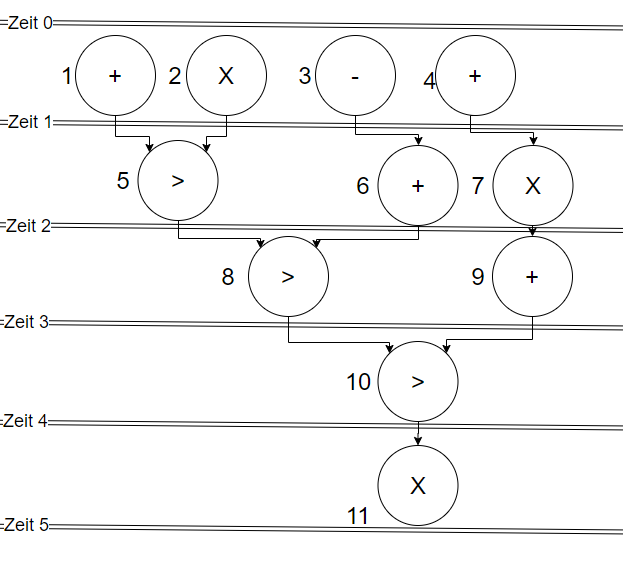
\includegraphics[scale=0.55]{fig_bsp_binding}}
\caption{Besipiel zur Bindung}
\label{fig.1}
\end{figure} 

Dem Bild ist zu entnehmen das in diesem beispiel für die zuordnung jeder Aufgabe zu einer Resource:11 Bauteile benötigt werden.
 Die sich aus 3 Multiplikationen = $r_1$ und aus 8 operationen für eine Arithmetisch logisch einheit $r_2$ ergibt.\\
\begin{tabular}[h]{ccc}
$v_i$&$\beta(v_i)$&$\gamma(v_i)$\\
$v_1$&$r_2$&1\\
$v_2$&$r_1$&1\\
$v_3$&$r_2$&2\\
$v_4$&$r_2$&3\\
$v_5$&$r_2$&4\\
$v_6$&$r_2$&5\\
$v_7$&$r_1$&2\\
$v_8$&$r_2$&6\\
$v_9$&$r_2$&7\\
$v_10$&$r_2$&8\\
$v_11$&$r_1$&3\\
\end{tabular}
Da es sich, um ein recht einfach zu überblickendes beispiel handelt, lässt sich durch einen geübten blick bereits erkennen wie eine Optimierung aussehen könnte. Im ersten Zeitslot ist abzulesen, das 3 Arithmetische operationen und eine Multiplikation durchgeführt werden, somit werden 3 ALU Einheiten und ein Multiplizierer benötigt.Im weiteren verlauf lässt sich unteranderem erkennen das in keinem weiteren zeitzlot mehr als 3 ALU einheiten gebraucht werden, deswegen ist dies auch unsere minimal benötigte anzahl an Resourcen dieses typs. Ganz genau deutlich wird dies durch eine veranschaulichung in einer tabelle.
\begin{tabular}[h]{ccc}
Zeitslot&ALU&Multiplizierer\\
1&3&1\\
2&2&1\\
3&2&0\\
4&1&0\\
5&0&0\\
\end{tabular}
\\Aus der Tabelle kann nun abgelesen werden, das 3 Resourcen des Typs ALU benötigt werden und 1 des Typs Mulitplizierer.\\
Übertragen auf die obere Tabelle ensteht nun folgendes Binding.\\
\begin{tabular}[h]{ccc}
$v_i$&$\beta(v_i)$&$\gamma(v_i)$\\
$v_1$&$r_2$&1\\
$v_2$&$r_1$&1\\
$v_3$&$r_2$&2\\
$v_4$&$r_2$&3\\
$v_5$&$r_2$&1\\
$v_6$&$r_2$&2\\
$v_7$&$r_1$&1\\
$v_8$&$r_2$&1\\
$v_9$&$r_2$&2\\
$v_10$&$r_2$&1\\
$v_11$&$r_1$&1\\
\end{tabular}
Somit wurden in diesem beispiel 5 Alu einheiten die einen anteil von $62,5\%$ ausmachen eingespart. Bei den Multiplizierern wurde die benötigten Resourcen auf $\frac{1}{3}$ reduziert.

%-Welche INstanz und welcher Ressourcentyp
%-connected die ressourcen und instanzen zu eioner bestimmten aufgabe 

\subsection{Sharing}
das sharing beschreibt zusammen mit dem Binding,  die effektive mehrfachnutzung der Ressourcen, welches der minimierung der verwendeten hardware dient und somit zu reduzierung von Flächen und kosten problemen beiträgt. wobei das ziel des Sharing die frage nach dem Alghoritmus zur optimerung ist und anschließend mit einem Binding endet. In dem Kapitel Binding wurde ein einfach im Kopf zu lösendes Beispiel gezeigt, leider bleibt es in der Realität nicht immer bei so einfach zu lösenden systemen, so dass da schnell der überblick verloren gehen kann und zudem ein system unter umständen nicht zu lösen wäre. Aus diesem grund befasst sich dass sharing mit der frage wie ein vorhandenes system effektiv optimiert werden kann.Zu den Verwendeten Alghoritmen zählen unter anderem aus dem breich der REsource Dominated Circuits das Register sharing, Multiport Memory Binding und das Bus sharing and Binding und für den bereich der general circuits, sind es Unconstrained minimum - Area Binding, Performance Constrained Binding und zu letzt Performance Directed Binding.   
\section{Grundlegendes}

\subsection{Kompatiblitäts- und Konfliktgraphen}
Als vorrausetzung, um überhaupt eine sinnvolle Bindung beziehungsweise Allokierung erzeugen zu können muss sich im 1. schritt einmal mit dem eigentlichen problem befasst werden. Um das Problem darstellen zu können wird ein Graph aufgestellt, der die eigenschaften der elemente beschreibt. Dieser Schritt ermöglicht die betrachtung der einzelnen operationen mit einander und stellt auf welche mit einander Kompatibel sind und welche ein kritisches verhalten zu einander aufweisen.\\
Zwei oder mehr Operationen sind mit einander Kompatibel und können an die Gleiche Resource gebunden werden wenn sie nicht mit einander Konkurrieren und wenn sie dem gleichen Resourcen-typen angehören\cite[S.231]{3}\\
Das bedeutet konkreit, dass aufgaben mit einander kompatibel sind, wenn sie nicht im gleichen Zeitslot neben einander anliegen und wenn sie des gleichen typs sind zum Beispiel Addierer.
Die entwicklung der ges graphensystems kann grundsätzlich über 2 ansätze erfolgen, zum einen kann ein Kompatiblitätsgraph oder Verträglichkeitsgraph entwickelt werden, dieser graph gibt an welche Operationen verträglich zu einander sind und somit keine probleme darstellen komplemäntar dazu lässt sich durch den Konflikt graphen angeben welche Operationen im konflik zu einander stehen und eine genauere betrachtung bedüfen.\\
Ein Ressourcen Verträglichkeitsgraf ist definiert durch $ G_+(V,E)$ in denen die Knoten durch $ V = \{v_i;i=1,2,...,n\}$ definiert werden und die Kanten durch $E = \{\{v_i,v_j\}i,j = 1,2,...,n\}$ Die Knoten stellen die Operationen an sich dar, wohingegen die Kanten die Kompatiblen Operationspaare angeben\cite[S.231]{3}.\\
Zusammen gefasst nach  Teich \cite[S. 181-182]{1} lassen sich folgende verträglichkeiten für den kompatiblitätsgraphen aufführen:\\

demnach ist eine \textbf{Schwache verträglichkeit} gegeben, wenn zwei knoten des Graphen
eines Grahen mit einander verbunden sind und des gleichen Types angehören also zum beispiel eine Addition und ein Vergleich, da beide durch eine Arithmetisch logische einheit Verarbeitet werden können.\cite{?}\\

\textbf{Ablaufplan verträglich} ist ein graph hingegen, wenn seine Knoten als erste bedingung vom gleichen typ sind, also wie bei der schwachen verträglichkeit zum Beispiel aus 2 operationen vom typ Multiplizierer. Zum zweoten muss die bediingung erfüllt sein, das die starzeit des ersten knoten vor der des zweiten knotens liegen muss. Das bedeutet, dass Knoten die Ablaufverträglich sind nicht in dem selben zeitslot ausgeführt werden dürfen, andernfalls wären sie nicht Ablaufplan vertträglich\cite{?}.\\

Als leztztes definiert sich die \textbf{Starke verträglichkeit}, durch zwei Knoten die wieder vom gleichen typ sind und zudem von einandern abhängig sind. Das bedeutet die beiden knoten sind in einem logischen strang durch einen pfad im ablaufplan mit einander verbunden.\cite{?}

Die Graphische umsetzunge des Verträglichkeitsgraphes mit dem Beispiel aus den vorherigen kapiteln sieht dann wie folgt aus: 
\begin{figure}[h]
\center{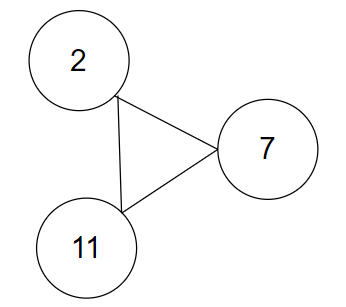
\includegraphics[scale=0.55]{fig_comp_mult}}
\caption{Verträglichkeitsgraph Mulitplizierer}
\label{fig.2}
\end{figure}\\
Aus den vorherigen kapiteln, wissen wir bereits, dass für die Optimierung der verschaltung nur ein Multiplizierer benötigt wird und genau das können wir in diesem beispil nun auch grafisch betrachten. Zu sehen ist, dass jeder knoten mit einer kante verbunden ist und somit sind alle Operationen mit einander Ablaufplan verträglich, weswegen der einsatz von nur einem Multiplizierer nun auch Optisch besser nachzuvollziehen ist.\\
\begin{figure}[h]
\center{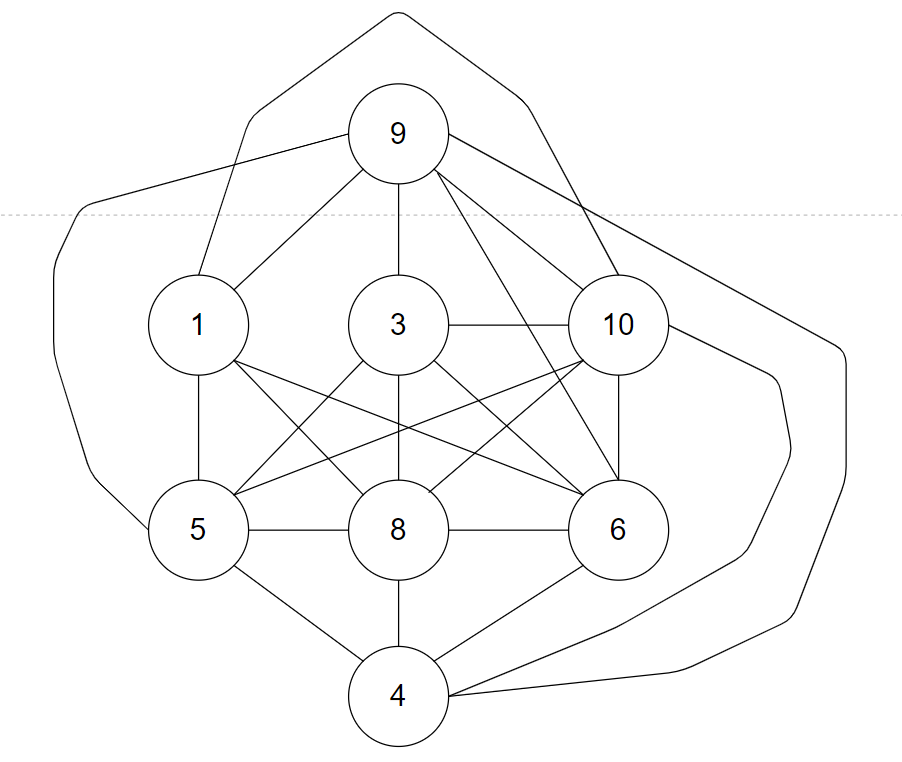
\includegraphics[scale=0.45]{fig_comp_alu}}
\caption{Verträglichkeitsgraph Arithmetisch logische einheit mit Cliquen}
\label{fig.4}
\end{figure}
Als nächsten schritt werden nun sogenannte Cliquen eingezeichnet, sie repräsentieren die zusammenfassung Mehrerer Operationen und zeigen ihre zusammenführung auf eine Komponente, so das für jede clique genau eine Komponente eingesetzt wird. Zu sehen ist, das Bei dem Verträglichkeitsgraphen in diesem Beispiel für die Mulitplizierer genau eine Clique eingezeichnet werden muss. Da mit steigender Komplexität der aufgabe, auch die Komplexität für das einzeichen der Cliquen steigt, bietet sich dieses verfahren leider nur für die anwendung an simple verschaltungen an, der Grund hierfür ist die klassifizierung dieses problems als NP-Hartes Problem.\cite[S.361]{2}\\
\begin{figure}[h]
\center{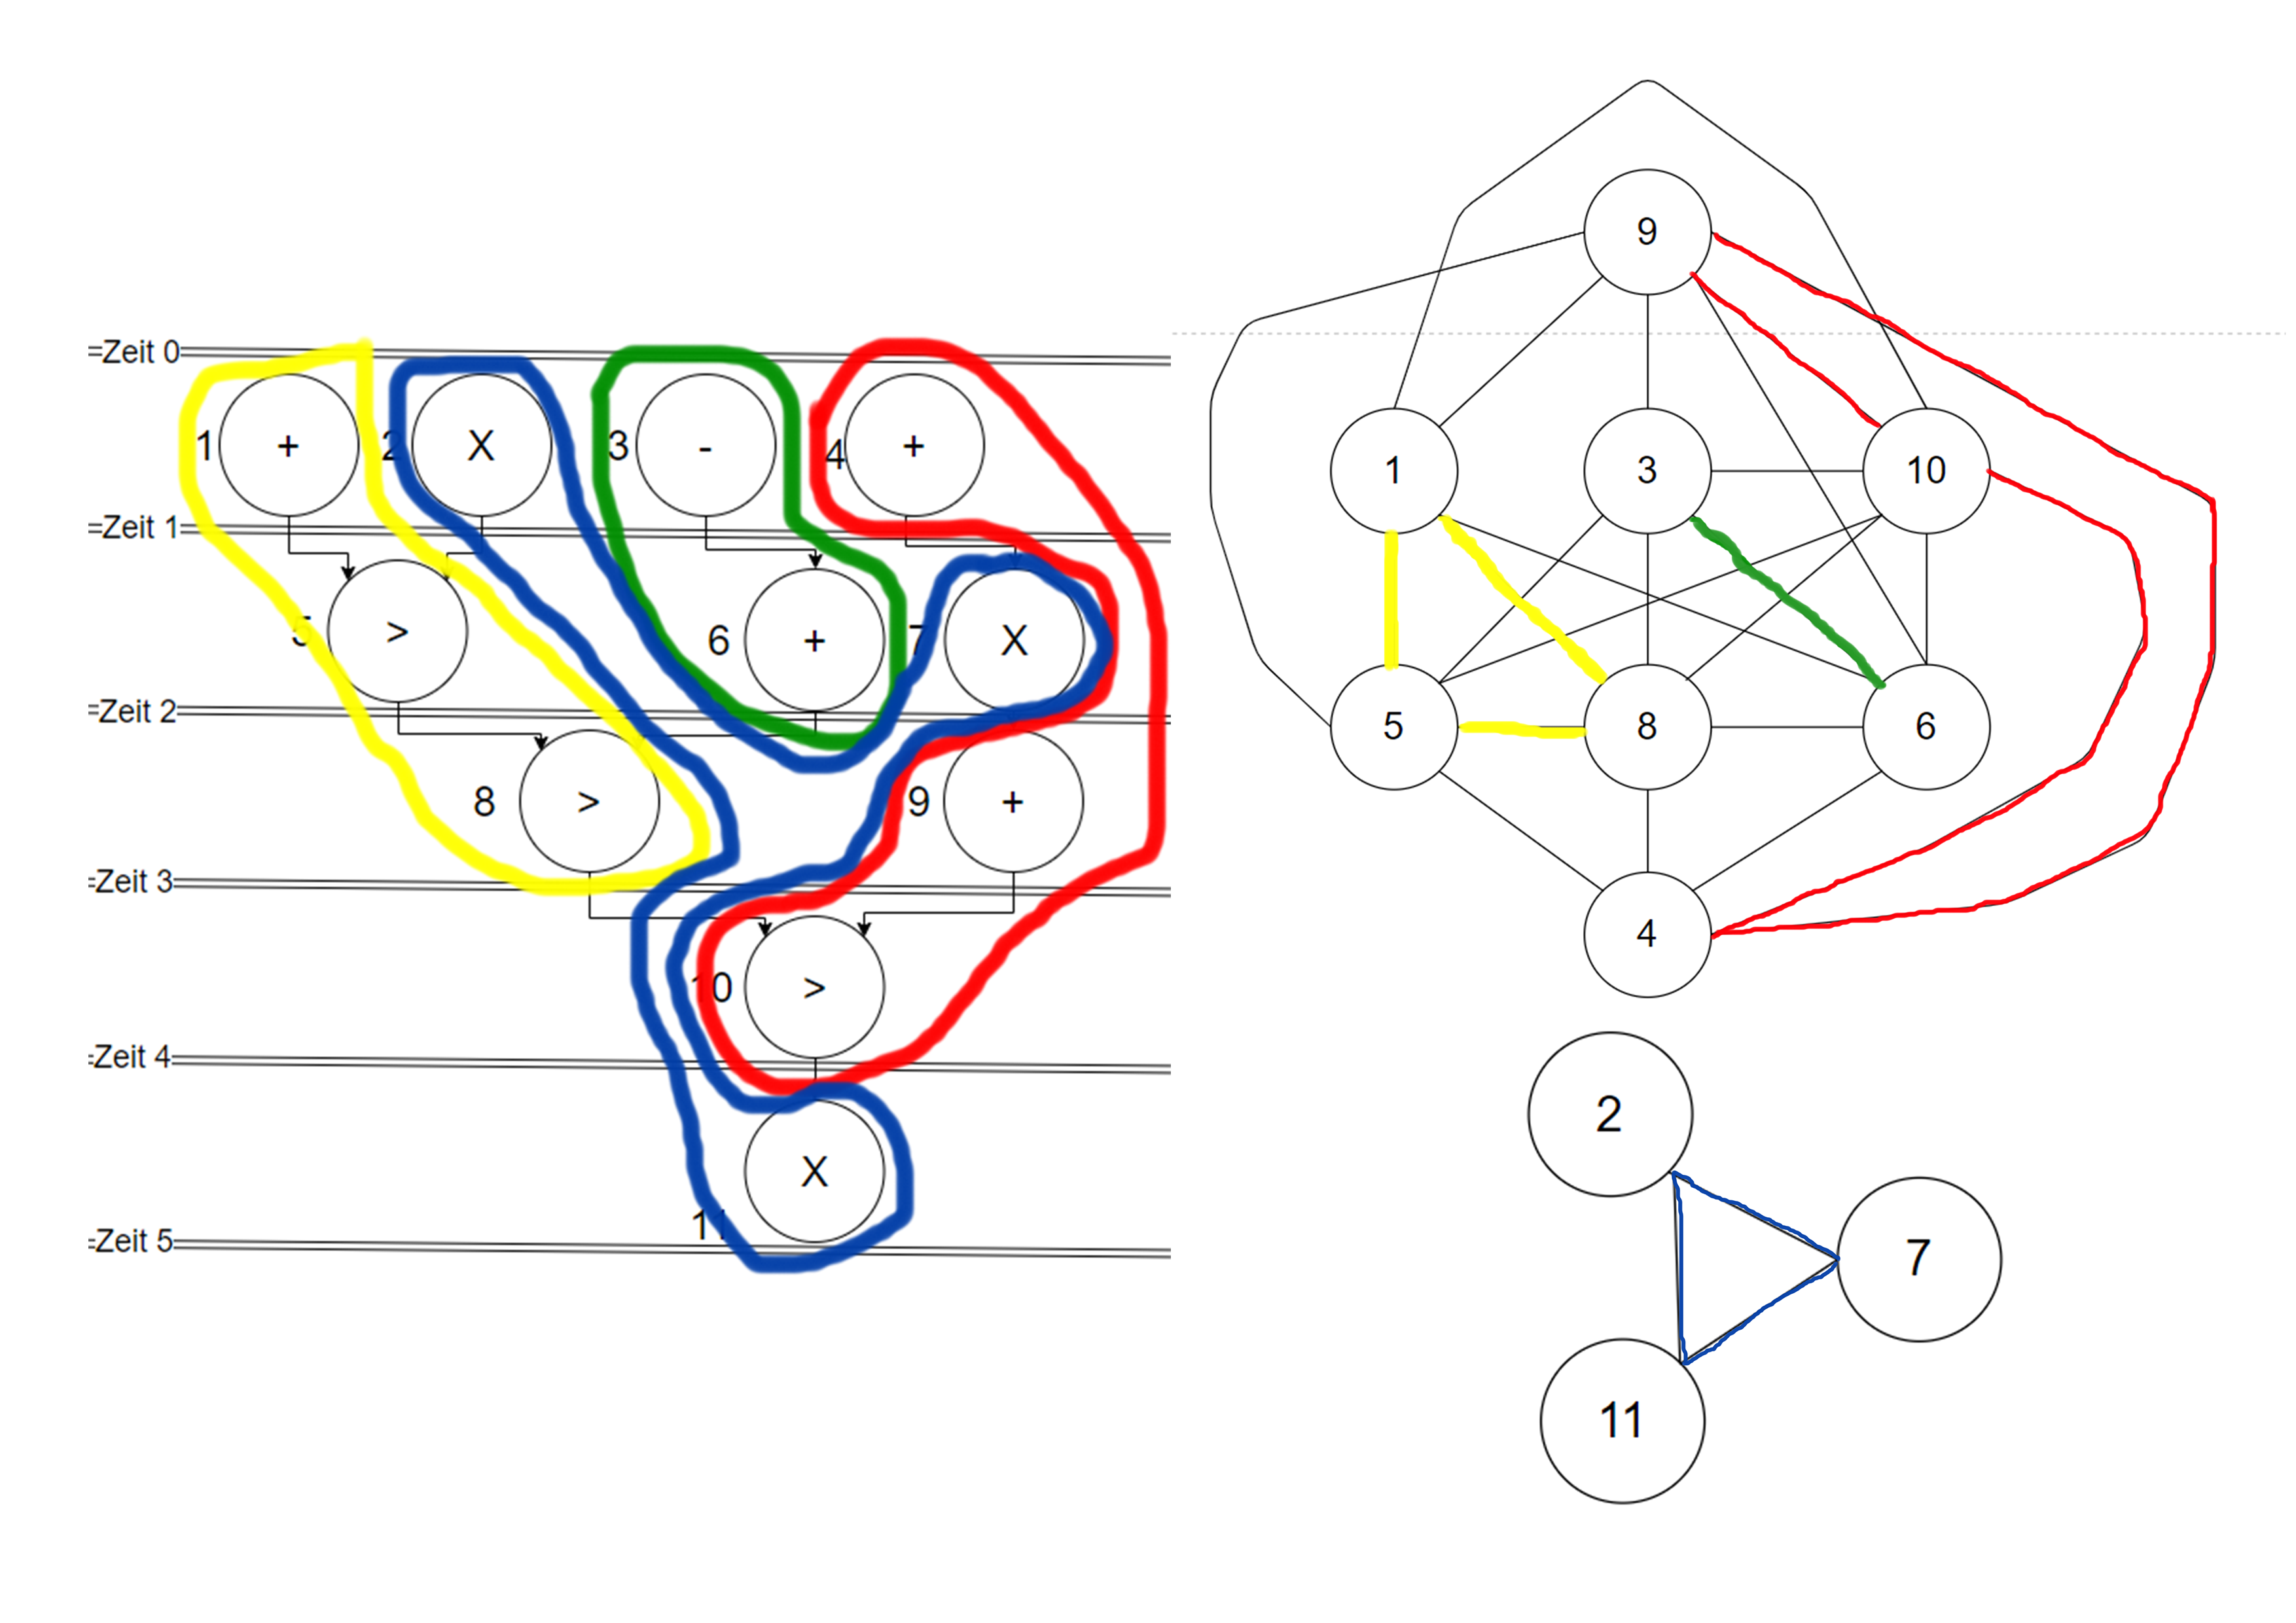
\includegraphics[scale=0.08]{fig_cliquen}}
\caption{Ablaufplan und verträglichkeitsgraphen mit Cliquenbildung}
\label{fig.3}
\end{figure}

%Graph zur betrachtung der Verträglichkeit einzelner Operationen
%zeigt auf einen bliock welche operationen mit einander kombiniert werden können %und welche nach folgenden regeln auf keinen fall kombiniert werden können

%-Schwach verträglich
%wenn vom gleichen ressourcentyp ?? 
%-Ablaufplan verträglich
%alternativ sind
%-Stark verträglich
%nicht gleichzeitig sind und mit einem gerichteten graph verbunden 




\subsection{Resource Dominated circuits}
Das "Sharing and Binding for Resource Dominated Circuits" (Verteilung und Bindung für Resourcen dominierte Schaltkreise) Bedeutet, im folgenden die umsetzung und kombinierung, des Wissens und der Grundlagen aus den voran gegangen Abschnitten.
Zur Erinnerung ist, das gesuchte ergebnis eine Bindung, das bedeutet eine zuordnung von tatsächlicher hardware und Operationen in denen eine maximale menge an Operationen einer minimalen menge an Hardware zugeordnet wird. hierfür ist im vorfeld zwingen festzustellen ob nicht druch andere dynamische umwelteinflüssen und anforderungen, eine grundsetzliche begrenzung der zur verfügung stehenden harware und fläche besteht (allokierung). Desweiteren, um überhaupt festellen zu können, welche operationen sich auf der selben hardware kombinieren lassen, muss ein Kompatiblitäts-/Konflikt-graph aufgestellt werden, mit dessen ergebnis sich operationen zu Cliquen bündeln lassen.
Leider ist die Lösung des vorliegenden problems nicht derart einfach, als einziges ziel lediglich die fläche und somit den preis der verschaltung zu optimieren, gerade in Echtezeitsystemen muss auch immer die aufmerksamkeit zu gleichen teilen auf der einhaltung der zeitlichen vorgaben bleiben.
Deswegen betrachtet das sharing and Binding für Resource Dominated Circuits, die Optimierung der Schaltung, bezüglich Fläche(Kosten) und  Latenz(Zeitschranken), mittels der Optimierung der wirkenden SChaltung mittels verminderung der eingesetzten Hardware und doppelnutzung dieser.\cite[S. 156]{3} 



%prüfen lassen ! 






\section{General Circuits}
Die betrachtung einer Schaltung unter dem aspekt der REsource Dominated Circuits ähnelt allerdings eher der betrachtung einer Idealen Komponete, als einer in denen auch störgrößen und andere umwelteinflüsse einer gewichteten zuwendung erfahren.
\subsection{Allgm.}
Aus diesem Grund wird für das Sharing and Binding for General Circuits ( Verteilung und Bindung für Generelle schaltkreise) nicht nur latenz und fläche der Operierenden Elektronik betrachtet, sondern auch derer, die steuernde und speichernde eigenschaften besitzen, zudem wird auch die verkabelung dieser nicht außen vor gelassen.\cite[S. 156]{3}
\subsection{Baugruppen}
 \subsubsection{Register}
 Da in schaltungen, wie sie in allen modernen systemen vorhanden sind, die über eine einfache input/output addition hinaus gehen Daten und werte über einen einzelnen zyklus hinaus gespeichert werden müssen, kommen in vielen schaltungen speicehrelemente zum einsatz beispielsweise müssen in Reglungs-Schaltungen werte gespeichert werden, die über mehrere zyklen zur verfügung stehen. \\
 Grundlegend verhält sich die bindung und das Teilen von registern ganz ähnlich zu den vorgängen bei normalen operatoren. Auch sind die vorgaben, beid denen REgister geteilt werden können gleich zu denen der Operatoren, das bedeutet Register können getielt werden, wenn sie nicht in konkurenz zu einander stehen, das beduetet wenn sie exklusiv zu einander stehen oder erst nach  einander auftreten. Nicht analog allerdings ist hier die definition der Lebenszeit einer variable und dementsprechend auch der register nutzung ist. Die lebenzeit ergibt sich nach De Micheli aus dem geburtszeitpunkt (\textit{former})  und dem Todeszeitpunkt (\textit{latter} einer variable. Der Geburtszeitpunkt ist der Zeitpunkt der erstellung durch das ergebnis einer Operation und der todeszeitpunkt ist als der späteste zeitpunkt anzunehmen in dem die Variable als input referenziert wird\cite[S. 240]{3}
Zur lösung der Registerbindung kann der Left-Edge Algorithmus verwendet werden \cite[S. 359]{2}\\
 \subsubsection{Steuerlogik}
 Unter der Berücksichtigung der steuerlogik kann sowohl für multiplexer, die ganz ähnlich zu den aufgezeigten vorgängen betrachtet werden kann, desweiteren auch Bussysteme bewertet werde nn hierzu wird das augenmerk auf zwei zu berücksichtigende komponenten gelegt. Als erstes wird der bus an sich selbst betrachtet, der einen fixwert zugeordet bekommt, einen sogenannten overhead.
 als Zweite komponente werden die Bustreiber aufgefürt, also die funktionseinheiten, die zur steuerung des busses fungieren. diese kann als verteilter multiplexer betrachtet werden, was eine berechnung von anzahl und verbraucht möglich macht.\cite[S. 157]{3}\\
 \subsubsection{Verkabelung}
 Als ein weiterer,nicht zu vernachlässigbarer bereich, gilt vor allem für das platzmanagement die benötigte Verdrahtung zur verbindung der plazierten bauteile. Hierbei ist zu beachten, das nun auch starke physikalische beeinflussung mit in die plazierung der komponenten mit einbezogen werden muss und sich somit wiederum auch auf die benötigte fläche ausbreitet, so müssen beispielsweise leitungen die betriebsspannung führen möglichst von empfindlichen busleitung räumlich fern gehalten werden.
Somit ist eine umumgehbarer vorrausetzung für die ermittlung des platzbedarfs, kenntnis über die strucktur der elemente , dazu zählen ihre größe, ihre anzah und ihre plazierung zudem ist auch die bindung der elemnete von bedeutung ,da diese einen direkten einfluss auf ihre verkabelung hat \cite[S.157]{3}
Zur berechnung ergibt sich, dass die länge der verdrautung proportional zur anzahl der einhgesetzen funktionsblöcke, hoch $\alpha$ ist, wobei $0 \leq \alpha \geq 1$ ist.\cite[S.157]{3}\\
 \subsubsection{kontroll einheiten}
 Da Signale zur steuerung von bausteinen unerlässlich sind und diese signake letzendlich den gleichen beschränkungen und einflüssen unterliegen wie datensignale kann es passieren, das diese steuersignale auf einem Kritischen pfad liegen und somit zu einem problem für den Programm ablauf werden.\\
 Eine möglichkeit der Optimierung, ist die reduzierung des ROM ( \textbf{R}ead \textbf{O}nly \textbf{M}emory)
dies ist möglich, wenn es sich um eine implementierung eines Microcode basierter Kontroll einheit handelt. Der vorgang sieht in diesem fall vor nicht eine sogenannte horizontale umsetzung eines des Microcodes, der eine eins zu eins verbindung von bits zu steuersignalen vorsieht, sondern die umsetzung in einer Vertikalen variante des Microcodes, der bits in gruppen zusammen fasst und demnach die menge der zu speichernden daten reduzieren kann.
\cite[S.371-372]{2}
Hart verdratete codierungen hingegen lassen sich nur durch ihre verschiedene bauweise optimieren und anpassen, wohingegen der gedanke der anpassung bedeutet, eine gewisse störsicherheit einzubiunden so werden in kritischen umgebungen, in denen es nicht zu sörsignalen kommen darf die einen bit kippen lassen würden gray code impule verwendet um in den nächsten zeitschritt zu springen.\cite[S.373]{2}
\section{Sharing and Binding for General Circuits}
\subsection{Unconstrained minimum - Area Binding}
%kann gelöst werden bei standart linearen solvern als nicht lineares sytsem mit linearen bedingungen 
%allerdings ist es nur fr kleine circuits wirklich effektiv
%modeliert mittels eines kompatiblitäts graphs mit gewichteten kanten
%das gesamte system kann in vile kleine untersysteme aufgeteilt werden so z.b als graph für adder und als graphen für multiplxer oder die steering logic
%ganz ähnlich also einer gewichteten clique, wobei die anzahl der cliquen die cliquen überdeckungszahl übersteigen kann da nicht maximale cliquen ausgewählt werden können
%2 problemme entstehen
%1. das gewichtete cliquen partionierungs problem hierfür werden heuristische algorithmen genutzt
Zur berechnung und Einschätzung der kosten, und somit der möglichkeit diese zu minimieren muss wie bereits in vden vorherigen kapiteln, festegestellt eine Möglichkeit geschaffen werden mehr als eine operation einer hardware komponente zuornden zu können. Hinzu gekommen ist nun auch die betrachtung der Steuerlogik, der Datenübertragung und der Verkablelung die ebenfalls einen nich unerheblichen einfluss auf die effizienz einer schaltung nehmen.Ganz Äquivalent wird nun auch unter berücksichtigung dieser versucht heraus zu finden, ob und in welchem rahmen diese verteilt werden können. Durch den umstand, das die vorgehenswise ähnlich zu der ist , die von der einfachen betrachtung ohne die steuerlogik bekannt ist, ergeben sich auch ganz ähnliche probleme bei der arbeit mit dieser.\\
Problematisch ist nun auch, dass auch in diesem fall mit steigender komplexität der Verschaltung das bestimmen eines Optimums zunehmend schwieriger wird. Deswegen wird versucht mittels bestimmter algorithmen, den Perfekten graphen zu finden. 
Da ein perfekter Graph, die annahme zulässt, das er in Polynomialzeit zeit berechenbar ist,kann angenommen werden das, das ein ergebnis in einer akzeptablen zeit zu erwarten ist. Für den fall, das sich der Perfekte graph in Polynomialzeit brechnen lässt, gilt auch, das sich all seine Parameter ebenfalls in akzeptabler zeit berechnen lassen\cite[S. 60]{6}.\\
Eine mögliche vorgehensweise ist, die kosten für z.b Multiplexer gleichmäßig über die operatoren zu verteilen\cite[S.247]{3}
Ermöglicht wird dies über eine gänzliche betrachtung der cliquen, denen ein set an kosten zugeordnet wird, das sich aus den kosten mengen ihrer knoten ergibt. Ihre gewichtung erhaält die clique durch die anzahl ihrer hinzu gefügten knoten. Die gesamtkosten wiederum ergeben sich aus der Summe der Cliquen, die zu einer partition zusammengefügt werden.\cite[S. 247]{3}\\
So kann eine formel für Multiplexer wie folgt aussehen:\\
\begin{center}
$area_{mux} = area_{mux}^{\Delta}(a-1)  $ \\und wird als:\\ $area_{M}^{0} + \sum_{i=1}^{a}area_{M}^{i}$\\ geschrieben\\  \cite[S. 247]{3}
\end{center}

Desweiteren kann ein Algorithmus nach Tseng und Siewiorek genutzt werden in dem Cliquen partioniert, also zusammengefasst werden. Das Ziel des Alorithmus ist es ungewichtete untergraphen zu erstellen, um im anschluss eine Optimierung erhalten zu können\cite[S. 247]{3}.
Erreicht wird dies durch das erkennen und auswählen des knotenpares mit den meisten Gemeinsamen Knoten die mittels einer Kante Verbunden sind, gesucht wird also das Paar mit den meisten gemeinsamen Nachbarn. Sobald das paar mit den meisten nachbarn gefunden wurde, werden diese zusammengeführt, nach der zusammenführung werden nun alle Kanten gelöscht, die nicht in Verbindung mit beiden zusammengeführten knoten stehen. Übrig bleiben demnach nur noch ein verbundenen knoten und alle kanten, die mit beiden knoten in verbindung standen. Dies kann solange durchgeführt werden, wie sich Partner für eine zusammen führung finden lassen, andernfals ist die erstellte clique maximal und kann abgespeichert , gegebenenfalls gefärbt und anschliessend geupdatet werden.Eine Aktualisierung des Graphen lässt sich mittels des Updating algorithmus nach Tseng und Siewiorek\cite[S.393]{5}durchführen, indem die Kanten, die zusammengeführt wuren, aus der liste der kanten entfernt werden und in eine liste der gelöschten kanten eingetragen wird, anschlieschend werden in einem zweiten schritt wird die anzahl der nächsten nachbarn und die anzahl der kanten die gelöscht werden müssen neu. 
 Abgeschlossen ist die cliquenpartionierung in dem moment, in dem sich keine kanten mehr in der kanten liste befinden\cite[S.248]{3}\cite[S.392-393]{5}.\\
Ein Graph ist in dem Moment Perfekt, wenn auch alle seine Untergraphen $H(G)$ folgende bedingung erfüllen. Ein Untergraph ist perfekt, wenn die Mächtigkeit seiner größten Clique gleich ist mit der Chromatischen zahl. $\omega(H) = \chi(H)$ Desweiteren muss die unabhängigkeitszahl $ \alpha(H)$, die angibt, welche Knoten nciht miteinandern durch ein kante verbunden sind, also in einem nicht adjazenten verhältnis stehen, ebenfalls gleich mit der anzahl an unabhängigen mengen, also der Zusammenhangszahl $(\kappa(H)$ gleich sein $\alpha(H) = \kappa(H)$\cite[S.507]{1}\cite[S.59 - 60 ]{6} Das bedeutet Konkret am besipeil der Voran gegangenen Algorithmen, dass versucht wird, einen graphen zu Optimieren, in dem der graph in Untergraphen zerlegt wird und für diese geprüft wird, ob ein Optimum vorliegt.
 \subsection{Performance Constrained Binding und Performance Directed Binding}
Neben der Optimierung der Kosten, durch reduktion der Eingesetzten Hardware, war es zwingend notwendig einen weiteren aspekt zu beobachten, da dieser direkt durch die mehrfachnutzung der hardwarekomponenten beeinflusst wird.
Da die reduzierung der benutzen hardware, auch immer einen direkten einfluss auf die zeit hat, die zur ausführung der aufgaben benötigt wird hat, beeinflusst auch die verbaute steuerelektronik, die verkabelung und die Daten haltung unmittelbar die ausführungszeit. Gerade Multiplexer wirken sich negativ auf die benötigte ausführungszeit aus, da eine direkte serielle 1 zu 1 verkabelung, immer schneller ist, als eine Gemulitplexte, in denen die übertragung zu gunsten von chipfläche und weniger verkabelung reduzuiert wird.\\

\section{Gleichnis,vorgestellter Algorithmen}
\section{Ausblick}

\begin{thebibliography}{00}
\bibitem{1} Jürgen Teich, Christian Haubelt, Digitale Hardware/Software-Systeme, Synthese und Optimierung, 2. Auflage,Springer,2007
\bibitem{2} Dr.Walter Lange, Prof.Dr.Martin Bogdan, Entwurf und Syntese von Eingebetteten Systhemen, Ein Lehrbuch,Oldenbourg Verlag München, 2013
\bibitem{3} Giovanni De Micheli, Synthesis and Optimization of Digital Circuits,McGraw-Hill, Inc. New York etc,1994
\bibitem{4} Martin Pieper, Mathematische Optimierung, Eine Einführung in die Kontinuierliche Optimierung mit Beispielen,Springer Spektrum,2017
\bibitem{5} Chia-Jeng Tseng, Daniel P. Siewiorek, Automated Synthesis of Data Paths in Digital Systems,IEEE Xplore, 1986
\bibitem{6} Graphentheoretische Konzepte und Algorithmen, Sven Oliver Krumke \& Hartmut Noltemeier, 3. Auflage,Springer Vieweg, 2012
\end{thebibliography}
\listoffigures
\listoftables
\vspace{12pt}


\end{document}
